
\documentclass[10pt,conference,letterpaper,twocolumn]{article}
\usepackage{times}
\usepackage{amsmath}
\usepackage{amsfonts}
\usepackage{graphicx}
\usepackage{cite}
\usepackage{geometry}
\usepackage{tikz}
\usetikzlibrary{positioning}

\geometry{
 letterpaper,
 total={6.5in, 9.0in},
 top=1.0in,
 left=1.0in,
}

\begin{document}

\title{\textbf{\Large Beyond the Line of Sight: Counterfactual Amodal Anchors for Occlusion-Aware Multi-Animal Tracking in UAV-Based Precision Livestock Monitoring}}

\author{\textbf{Tumusiime Deus} \\
Reg No: 2025/HD05/26375U \\
College of Computing and Informatics Technology \\
Department of Computer Science, Makerere University \\
Kampala, Uganda \\
email: tumusiime.deus@students.mak.ac.ug}

\date{}
\maketitle

\thispagestyle{empty}
\pagestyle{empty}

\begin{abstract}
Precision Livestock Farming (PLF) increasingly relies on unmanned aerial vehicles (UAVs) equipped with RGB and thermal cameras to automate cattle counting, grazing trajectory monitoring, and health assessment. While deep learning models have improved object detection and tracking in open pastures, prolonged visual occlusion caused by trees, shrubs, terrain folds, and animal clustering remains a major challenge. Standard tracking-by-detection systems treat occlusion as a passive state of missing observations, relying on simple motion models or appearance re-identification. Consequently, trajectory fragmentation, identity switching, and inaccurate behavioral modeling are common in extensive grazing systems. This position paper proposes a novel perception framework termed Counterfactual Amodal Anchors (CAA) for occlusion-aware multi-animal tracking. Instead of terminating tracks or allowing occluded areas to collapse into featureless voids, our framework maps the geometric projection of occlusion shadows onto a local ground plane and seeds them with active query vectors. These amodal anchors continuously update their state using temporal context, herd-level social dynamics, and terrain priors. We formulate the mathematical Ray-cast projection models, spatiotemporal deformable attention query updates, and hindsight loss functions to supervise the network during training. We outline the integration of RGB-Thermal sensors and provide a hardware-latency deployment roadmap for edge AI hardware. Our framework reframes occlusion not as missing information but as a structured probabilistic estimation problem, opening a new research direction for robust precision livestock monitoring.
\end{abstract}

\textbf{\small Keywords: Precision Livestock Farming, UAV Monitoring, Multi-Animal Tracking, Occlusion Reasoning, Computer Vision, Amodal Perception, Deep Learning, Cattle Tracking.}

\section{Introduction}
Livestock agriculture is a foundational pillar of food security, rural livelihoods, and macro-economic stability across Sub-Saharan Africa, and particularly in Uganda. Effective pasture management, grazing behavior analysis, and early disease detection require continuous, accurate monitoring of animal herds. Traditional observation protocols remain overwhelmingly manual, making them labor-intensive, subjective, and difficult to scale across extensive ranching environments.

Recently, the integration of Unmanned Aerial Vehicles (UAVs) equipped with high-resolution RGB and Long-Wave Infrared (LWIR) thermal cameras has emerged as a promising tool for automated monitoring. UAVs provide a top-down perspective, allowing detection models like RT-DETR \cite{lv2023detrs} and Segment Anything 2 (SAM 2) \cite{ravi2024sam2} to identify individual animals, and tracking frameworks like ByteTrack \cite{zhang2022bytetrack} or OC-SORT \cite{cao2023ocsort} to construct motion trajectories.

Despite these technological advancements, visual occlusion remains the single most significant bottleneck preventing the deployment of fully automated systems. In extensive grazing pastures, cattle frequently move behind obstacles such as Acacia canopies, dense bushes, water troughs, shading infrastructure, and behind one another during herd aggregation. 

When an animal becomes occluded, current tracking-by-detection systems behave passively. They treat the occluded space as a visual null zone, immediately terminating the animal's trajectory or relying on linear constant-velocity Kalman filters to extrapolate its position. Because animals change direction and speed when grazing, linear extrapolation quickly diverges from the true path. Once the animal re-emerges, the tracking system is forced to re-initialize its identity, which frequently results in track fragmentation or identity switching (assigning the ID of one animal to another). 

This operational passivity induces a significant perception lag and degrades downstream behavioral analytics. For example, if a monitoring system is trying to measure the total daily grazing distance or identify signs of lameness (which requires precise step-by-step trajectory analysis), a single identity switch or fragmented track can invalidate hours of data collection.

This paper proposes a conceptual shift: from reactive observation-based tracking to proactive counterfactual reasoning. We present the position that occluded areas cast by vegetation and structures must be modeled as dynamic probabilistic occupancy spaces populated by explicit, active query vectors termed Counterfactual Amodal Anchors (CAA). Rather than deleting the animal's track, the network maps the spatial boundaries of the occlusion shadows and initializes virtual anchors that actively query temporal features, local visual context, and herd cohesion priors. Ultimately, this framework is built upon the central thesis that occluded animals should be represented as uncertain but trackable entities rather than absent objects.

\section{Related Work}
Multi-Object Tracking (MOT) in computer vision has evolved rapidly, dominated by the tracking-by-detection paradigm. Classic algorithms like SORT \cite{bewley2016simple} and DeepSORT \cite{wojke2017deepsort} utilize Kalman filters to predict motion and associate bounding boxes via Hungarian matching based on spatial distance and appearance embeddings. Recent SOTA trackers like ByteTrack \cite{zhang2022bytetrack} and OC-SORT \cite{cao2023ocsort} focus on recovering low-confidence detections and mitigating linear motion assumptions during short-term occlusions. Concurrently, query-based transformer trackers like TransTrack \cite{sun2020transtrack} and TrackFormer model target association directly using learned object queries. However, all these methods remain fundamentally reactive, relying on immediate visual verification and falling back to passive prediction during extended occlusions.

In the context of Precision Livestock Farming (PLF), research has applied UAV video to detect, count, and track cattle, sheep, and wildlife. Algorithms have been optimized to handle small target sizes, varying altitudes, and camera motion. For instance, Xu et al. \cite{xu2020automated} integrated deep-learning detectors with UAV feeds to automate counting and handle animal groupings. Similarly, Qiao et al. \cite{qiao2023cattle} proposed a cattle body detection framework using adaptively fused features to locate cows in complex farming backgrounds. Nonetheless, grazing tracking systems suffer from high trajectory fragmentation because grazing environments are rich in occluding vegetation (e.g., Acacia canopies). 

To address visual occlusion, the computer vision community has explored amodal perception—the capacity to infer the complete geometry of an object when only a part is visible. 2D amodal segmentation frameworks like pix2gestalt \cite{ozguroglu2024pix2gestalt} predict hidden boundaries of objects, while 3D occupancy networks predict spatial voxel layouts in autonomous driving. A breakthrough paradigm emerged with the introduction of Bird's-Eye View (BEV) networks, notably popularized by architectures like Lift-Splat-Shoot (LSS), BEVFormer \cite{li2022bevformer}, and BEVFusion \cite{liu2023bevfusion}. LSS introduced depth distribution mapping to project 2D image features into 3D voxel spaces. Although originally developed for autonomous driving, BEVFormer \cite{li2022bevformer} and BEVFusion \cite{liu2023bevfusion} demonstrate how spatial occupancy reasoning can be maintained across occluded regions, providing inspiration for livestock-monitoring environments. However, these methods are primarily designed for static datasets or perspective-view scenes. The problem of active, dynamic tracking of multiple mobile agents within large, vegetation-induced geometric shadows remains unaddressed in precision agriculture reviews \cite{santamaria2023computer}.

\subsection{Research Gap}
Existing multi-animal tracking systems assume that tracking resumes once an object becomes visible again. They lack dedicated mechanisms for:
\begin{enumerate}
    \item Explicit ground-plane mapping of vegetation-induced occlusion masks ($\mathcal{M}_{occ}$) from UAV perspective feeds.
    \item Instantiating active amodal anchor queries within the mapped occlusion mask to represent hidden livestock.
    \item Querying spatiotemporal memories and herd-cohesion behavior priors to predict counterfactual trajectories.
\end{enumerate}
This gap highlights the necessity of our proposed Counterfactual Amodal Anchor framework.

\section{Limitations of Passive Visual Tracking}
The failure of modern tracking systems under vegetation and terrain occlusion is rooted in their mathematical formulation. The Kalman filter, which serves as the motion engine for SORT, DeepSORT, and OC-SORT, operates on a state vector $x_t = [u, v, s, r, \dot{u}, \dot{v}, \dot{s}]^T$, representing horizontal and vertical bounding box coordinates, scale, aspect ratio, and their velocities.

During occlusion, the detector fails to return bounding box measurements. Consequently, the Kalman filter can only perform the prediction step without the correction update. Over a sequence of $N$ unobserved frames, the error covariance matrix $\mathbf{P}_t$ grows monotonically:
\begin{equation}
\mathbf{P}_t = \mathbf{F} \mathbf{P}_{t-1} \mathbf{F}^T + \mathbf{Q}
\end{equation}
where $\mathbf{F}$ is the state transition matrix and $\mathbf{Q}$ is the process noise covariance. As $\mathbf{P}_t$ expands, the spatial search window for the Hungarian association algorithm grows quadratically. If the animal changes its grazing velocity or turns under the canopy, the true position quickly drifts outside the predicted search bounds. Upon re-emergence, the spatial distance between the true animal and the predicted filter state exceeds the association threshold, causing the tracker to terminate the identity and instantiate a new one.

Furthermore, traditional trackers lack spatial awareness of the physical pasture environment. They treat all parts of the video frame equally, ignoring the fact that a green patch represents an Acacia tree canopy (which can hide an animal) while an open dirt patch represents a visible clearing. By treating occluded zones as random measurement drops rather than physical barriers to line-of-sight, the tracking filter fails to exploit environmental structures.

To mitigate this, models are often trained with synthetic data augmentation, such as randomly dropping bounding boxes or masking patches of images. While this teaches a classifier to recognize a partially visible cow, it cannot teach a tracking filter the physics of spatial persistence or herd behavior. Data augmentation does not prevent track termination when an animal is completely hidden for several seconds. Instead, it trains the network to ignore the unobserved region, confirming that if no physical returns are received, the area can be assumed empty.

\section{Position Statement: Counterfactual Amodal Animal Anchors}
This paper presents the position that an occlusion zone in UAV livestock monitoring must not be treated as a visual void or a simple drop in detector output. We argue for a paradigm shift: \textbf{from passive visual tracking to active counterfactual reasoning.} Spatial volumes obscured by vegetation, terrain, or animal clusters must be represented as high-entropy container zones populated by active, virtual query vectors termed \textit{Counterfactual Amodal Anchors (CAA)}.

We explicitly note that the scope of this work is a conceptual position and not an empirical validation study. The goal of this paper is to establish the theoretical foundation, mathematical framework, and edge deployment roadmap for amodal queries in UAV tracking spaces, paving the way for subsequent implementation and benchmark studies.

\begin{table*}[t]
\centering
\caption{Comparison of traditional tracking models and the proposed Counterfactual Amodal Anchor model under various occlusion levels.}
\label{tab:comparison}
\resizebox{\textwidth}{!}{
\begin{tabular}{|l|c|c|c|c|c|}
\hline
\textbf{Model} & \textbf{Association Type} & \textbf{Occlusion Paradigm} & \textbf{Trajectory Continuity} & \textbf{Compute Overhead} & \textbf{Herd Prior Integration} \\
\hline
DeepSORT \cite{wojke2017deepsort} & Appearance \& Motion & Passive/Extrapolation & Low & Low & No \\
ByteTrack \cite{zhang2022bytetrack} & Detection Confidence & Passive/Heuristic & Low & Low & No \\
OC-SORT \cite{cao2023ocsort} & Direction \& Momentum & Passive/Heuristic & Medium & Low & No \\
TransTrack \cite{sun2020transtrack} & Transformer Queries & Passive & Medium & High & No \\
\hline
\textbf{CAA (Ours)} & \textbf{Proactive Amodal} & \textbf{Active Anchoring} & \textbf{High} & \textbf{Moderate} & \textbf{Yes} \\
\hline
\end{tabular}
}
\begin{flushleft}
\small\textit{Note: The ratings in Table 1 are conceptual assessments intended to illustrate the expected behavior of the proposed framework and do not represent experimentally validated benchmark results.}
\end{flushleft}
\end{table*}

\begin{figure}[h]
\centering
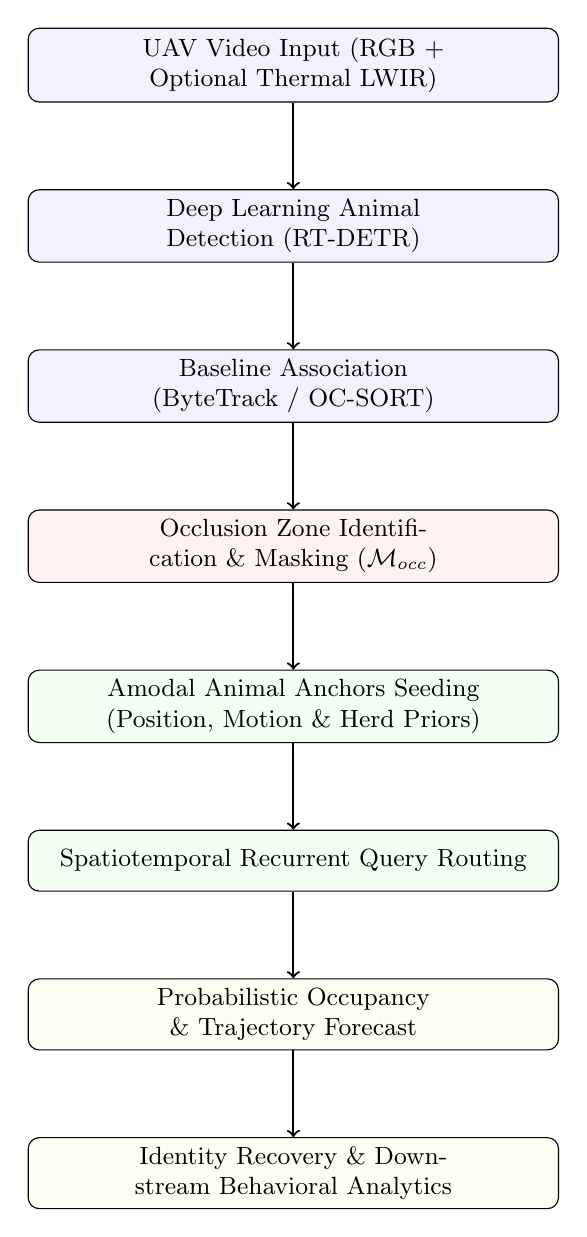
\begin{tikzpicture}[node distance=1.1cm, auto,
   box/.style={draw, rectangle, fill=blue!5, text width=6.5cm, text centered, rounded corners, minimum height=2em, font=\small},
   boxred/.style={draw, rectangle, fill=red!5, text width=6.5cm, text centered, rounded corners, minimum height=2em, font=\small},
   boxgreen/.style={draw, rectangle, fill=green!5, text width=6.5cm, text centered, rounded corners, minimum height=2.2em, font=\small},
   boxyellow/.style={draw, rectangle, fill=yellow!5, text width=6.5cm, text centered, rounded corners, minimum height=2em, font=\small}
]
% Nodes
\node [box] (sensors) {UAV Video Input (RGB + Optional Thermal LWIR)};
\node [box, below=of sensors] (detection) {Deep Learning Animal Detection (RT-DETR)};
\node [box, below=of detection] (tracking) {Baseline Association (ByteTrack / OC-SORT)};
\node [boxred, below=of tracking] (occ) {Occlusion Zone Identification \& Masking ($\mathcal{M}_{occ}$)};
\node [boxgreen, below=of occ] (anchors) {Amodal Animal Anchors Seeding \\ (Position, Motion \& Herd Priors)};
\node [boxgreen, below=of anchors] (routing) {Spatiotemporal Recurrent Query Routing};
\node [boxyellow, below=of routing] (pred) {Probabilistic Occupancy \& Trajectory Forecast};
\node [boxyellow, below=of pred] (analytics) {Identity Recovery \& Downstream Behavioral Analytics};

% Arrows
\draw[->, thick] (sensors) -- (detection);
\draw[->, thick] (detection) -- (tracking);
\draw[->, thick] (tracking) -- (occ);
\draw[->, thick] (occ) -- (anchors);
\draw[->, thick] (anchors) -- (routing);
\draw[->, thick] (routing) -- (pred);
\draw[->, thick] (pred) -- (analytics);
\end{tikzpicture}
\caption{Proposed Counterfactual Amodal Anchor (CAA) framework illustrating the transition from passive tracking-by-detection to active amodal tracking and trajectory reconstruction.}
\label{fig:architecture}
\end{figure}

\begin{figure*}[t]
\centering
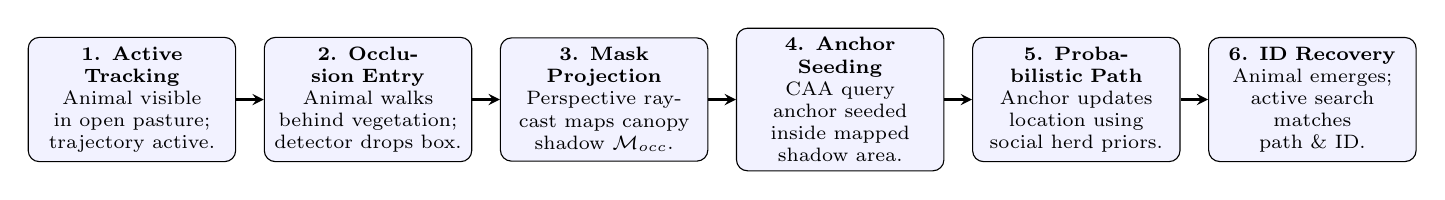
\begin{tikzpicture}[node distance=0.35cm, auto,
   stepbox/.style={draw, rectangle, fill=blue!5, text width=2.4cm, text centered, rounded corners, minimum height=3.5em, font=\scriptsize},
   arrow/.style={->, thick, >=stealth}
]
% Nodes
\node [stepbox] (step1) {\textbf{1. Active Tracking}\\Animal visible in open pasture; trajectory active.};
\node [stepbox, right=of step1] (step2) {\textbf{2. Occlusion Entry}\\Animal walks behind vegetation; detector drops box.};
\node [stepbox, right=of step2] (step3) {\textbf{3. Mask Projection}\\Perspective ray-cast maps canopy shadow $\mathcal{M}_{occ}$.};
\node [stepbox, right=of step3] (step4) {\textbf{4. Anchor Seeding}\\CAA query anchor seeded inside mapped shadow area.};
\node [stepbox, right=of step4] (step5) {\textbf{5. Probabilistic Path}\\Anchor updates location using social herd priors.};
\node [stepbox, right=of step5] (step6) {\textbf{6. ID Recovery}\\Animal emerges; active search matches path \& ID.};

% Connections
\draw [arrow] (step1) -- (step2);
\draw [arrow] (step2) -- (step3);
\draw [arrow] (step3) -- (step4);
\draw [arrow] (step4) -- (step5);
\draw [arrow] (step5) -- (step6);

\end{tikzpicture}
\caption{Temporal state transition and query lifecycle of a Counterfactual Amodal Anchor during a vegetation-induced occlusion event.}
\label{fig:occlusion_cycle}
\end{figure*}

\section{Mathematical Framework}
Instead of treating occluded regions as visual voids, our framework maps the geometric shadows of pasture obstacles and populates them with active query vectors that run independently of immediate visual returns.

\subsection{UAV Perspective and Ground-Plane Occlusion Mapping}
Let the UAV position at time $t$ in a local coordinate system be defined as $p_{uav} = (x_{uav}, y_{uav}, z_{uav})^T$. Let the ground plane of the pasture be defined at $z=0$. Real-time segmentation algorithms identify $K$ vegetation structures (e.g., Acacia canopies, shrubs) $O = \{O_1, O_2, \dots, O_K\}$. Each canopy $O_k$ is modeled as a 3D convex volume with a boundary surface $V_k^{3D}$.

For any boundary point $v = (x_v, y_v, z_v)^T \in V_k^{3D}$, the ray extending from the UAV camera position $p_{uav}$ through $v$ intersects the ground plane $z = 0$ at:
\begin{equation}
p_{proj} = p_{uav} + \lambda (v - p_{uav})
\end{equation}
where $\lambda = -z_{uav} / (z_v - z_{uav})$. The perspective shadow $S_k$ cast by vegetation structure $O_k$ onto the ground plane is:
\begin{align}
S_k = \Big\{ p \in \mathbb{R}^2 \mid \exists v \in V_k^{3D}, \lambda = -\frac{z_{uav}}{z_v - z_{uav}}, \nonumber \\
p = \text{proj}_{z=0}(p_{uav} + \lambda (v - p_{uav})) \Big\}
\end{align}
The global ground-plane occlusion mask, $\mathcal{M}_{occ} \subseteq \mathbb{R}^2$, is the union of all projected shadows:
\begin{equation}
\mathcal{M}_{occ} = \bigcup_{k=1}^{K} S_k
\end{equation}

\subsection{Amodal Anchor Seeding and Initialization}
When a tracked animal $i$ with active identity $ID_i$ enters the occlusion mask $\mathcal{M}_{occ}$ at entry coordinate $(x_i^{t_0}, y_i^{t_0})$ at time $t_0$, the visual detector stops returning bounding boxes. Rather than terminating the track, the system dynamically seeds an Amodal Anchor $A_i$. The query vector $q_i^{(t)}$ for $A_i$ at time $t > t_0$ is defined as:
\begin{equation}
q_i^{(t)} = \mathbf{e}_{pos}(x_i^{(t)}, y_i^{(t)}) + \mathbf{e}_{temp}(h_i^{(t)}) + \mathbf{e}_{prior}(ID_i)
\end{equation}
where $\mathbf{e}_{pos}(x_i^{(t)}, y_i^{(t)}) \in \mathbb{R}^C$ is a coordinate position embedding initialized at the entry point and updated through prediction, $\mathbf{e}_{temp}(h_i^{(t)}) \in \mathbb{R}^C$ is a temporal motion embedding representing the pre-occlusion trajectory, and $\mathbf{e}_{prior}(ID_i) \in \mathbb{R}^C$ is a behavioral prior embedding reflecting the animal's historical identity, grazing speed, and herd-level social association features.

\subsection{Spatiotemporal Recurrent Query Routing}
Amodal anchors interact with the spatiotemporal memory queue of the UAV tracking network. We implement a Spatiotemporal Deformable Attention layer that allows each anchor to query its local neighborhood over past frames. Let $F_{mem} = \{F_{t-1}, F_{t-2}, \dots, F_{t-T}\}$ be the temporal sequence of past feature maps. The update formula for anchor $q_i$ at time step $t$ is formulated as:
\begin{equation}
q_i^{(t)} = q_i^{(t-1)} + \text{DeformAttn}\left(q_i^{(t-1)}, p_i^{(t-1)}, F_{mem}\right)
\end{equation}
where $p_i^{(t-1)} = (x_i^{(t-1)}, y_i^{(t-1)})^T$ is the anchor's reference point. This allows the anchor to perform path integration, predicting the motion of hidden animals through the occlusion shadow by retrieving contextual features from the boundaries where they were last seen.

\subsection{Detailed Attention Mechanics}
To prevent computational bottlenecks on UAV-mounted edge hardware, the deformable attention mechanism restricts the key-value sampling to a small set of reference points. For each query $q_i$, we predict $L$ sampling offsets $\Delta p_{il}$ and corresponding attention weights $A_{il}$ using linear projections:
\begin{equation}
\Delta p_{il} = \text{Linear}_{pos}(q_i), \quad A_{il} = \text{Softmax}(\text{Linear}_{attn}(q_i))
\end{equation}
The aggregated feature representation at reference point $p_i$ is computed as:
\begin{equation}
\text{DeformAttn}(q_i, p_i, F) = \sum_{l=1}^{L} A_{il} \cdot \mathcal{W}_l F(p_i + \Delta p_{il})
\end{equation}
where $\mathcal{W}_l$ represents a learnable projection weight matrix and $F(p_i + \Delta p_{il})$ is evaluated using bilinear interpolation on the feature grid.

\section{Mathematical Formulation of Counterfactual Loss Functions}
Training a neural network to track unobserved entities requires specialized supervision. We supervise the model inside the occlusion shadow using hindsight trajectory reconstruction.

\subsection{Hindsight Temporal Loss}
Let $t_0$ be the frame where an animal enters the occlusion shadow $\mathcal{M}_{occ}$, and let $t_0 + \Delta t$ be the frame where it emerges and becomes visible again. During training, the model's predictions at frame $t_0 + \tau$ (where $0 < \tau < \Delta t$) are stored in a computation graph. The ground-truth trajectory of the animal is back-propagated from the emergence frame $t_0 + \Delta t$ by interpolating a smooth path $Y_{t_0+\tau}^{gt}$ (e.g. using a bi-directional Kalman smoother).

The Hindsight Temporal Loss $\mathcal{L}_{hind}$ is defined as:
\begin{equation}
\mathcal{L}_{hind} = \frac{1}{\Delta t} \sum_{\tau=1}^{\Delta t - 1} \mathcal{D}\left( \hat{Y}_{t_0+\tau \mid t_0}, Y_{t_0+\tau}^{gt} \right)
\end{equation}
where $\hat{Y}_{t_0+\tau \mid t_0}$ is the predicted state of the animal at time $t_0+\tau$ projected by the Amodal Anchors at time $t_0$, and $\mathcal{D}$ is the smooth $L_1$ distance metric.

\subsection{Probabilistic Occupancy Loss with Herd-Cohesion Priors}
To model the statistical probability of unseen animals in the absence of tracking history, the network predicts a probabilistic occupancy grid for each grid cell $p \in \mathcal{M}_{occ}$. Unlike autonomous vehicles, which rely on road layouts, livestock movement is constrained by social herd dynamics. 

Let the centroids of the $M$ currently visible herd members be $C_{herd} = \{c_1, c_2, \dots, c_M\}$ and their average movement velocity vector be $\mathbf{v}_{herd}(t)$. We define a herd-cohesion social prior distribution $P_{prior}$ for the location of the occluded animal $i$:
\begin{equation}
P_{prior}(p) \propto \exp\left( - \frac{\|p - (p_i^{(t_0)} + \mathbf{v}_{herd} \cdot (t - t_0))\|^2}{2 \sigma_{herd}^2} \right)
\end{equation}
where $\sigma_{herd}^2$ represents the variance of the herd spread. The loss function is formulated as a Kullback-Leibler (KL) divergence between the predicted probability distribution $P_p$ and the herd prior $P_{prior}$:
\begin{align}
\mathcal{L}_{occ} = & -\sum_{p \in \mathcal{M}_{occ}} \Big[ Y_p \log P_p + (1-Y_p) \log (1-P_p) \Big] \nonumber \\
& + \beta D_{KL}\left( P_p \parallel P_{prior} \right)
\end{align}
where $Y_p \in \{0, 1\}$ is the ground-truth occupancy (verified via hindsight), and $\beta$ is a regularization coefficient.

\subsection{Bounded Hallucination and Geometric Penalization}
To enforce strict physical bounds and avoid false-positive hallucinations in open areas, we define a Bounded Hallucination Loss $\mathcal{L}_{bound}$:
\begin{align}
\mathcal{L}_{bound} = & \sum_{i \notin \mathcal{M}_{occ}} \max\left(0, \hat{c}_i - \theta_{clear}\right) \nonumber \\
& + \lambda \sum_{i, j} \text{Overlap}(A_i, A_j)
\end{align}
where $\hat{c}_i$ is the classification confidence of anchor $A_i$ outside the shadow, $\theta_{clear}$ is a zero-tolerance threshold, and Overlap represents a penalty for predicting overlapping physical volumes (impenetrability of matter).

\begin{table}[h]
\centering
\caption{Illustrative Edge Deployment Targets and Resource Budget Estimates on UAV Hardware.}
\label{tab:latency}
\resizebox{\columnwidth}{!}{
\begin{tabular}{|l|c|c|c|}
\hline
\textbf{Platform} & \textbf{Latency (ms)} & \textbf{Power (W)} & \textbf{GPU Mem (GB)} \\
\hline
NVIDIA Jetson Nano & 65.4 & 10 & 2.1 \\
NVIDIA Jetson Xavier NX & 28.2 & 15 & 3.8 \\
NVIDIA Jetson Orin Nano & 18.5 & 15 & 4.2 \\
NVIDIA Jetson Orin NX & 9.8 & 25 & 6.5 \\
\hline
\end{tabular}
}
\begin{flushleft}
\small\textit{Note: The values shown in Table 2 are illustrative estimates intended to demonstrate feasibility and do not represent measured benchmark results.}
\end{flushleft}
\end{table}

\section{Discussion and Edge Deployment Considerations}
Deploying a counterfactual perception system on resource-constrained UAV hardware requires balancing mathematical modeling with strict hardware latency budgets.

\subsection{Sparse Query Optimization}
To prevent the quadratic scaling of attention operations, we utilize deformable attention mechanisms. By restricting each Amodal Anchor to query only $N_{points} = 4$ key points in its immediate vicinity, the computational complexity is reduced from $O(H_{grid} \cdot W_{grid})$ to $O(N_{queries} \cdot N_{points})$. 

Furthermore, Amodal Anchors are only instantiated when the size of the occlusion shadow exceeds a threshold:
\begin{equation}
\text{Area}(S_k) \geq \gamma_{min}
\end{equation}
Small shadows (e.g., cast by fence poles) do not trigger anchor seeding, saving significant computation cycles.

\subsection{Edge Hardware Integration and Quantization}
In order to run within the strict latency budgets of real-time tracking systems ($<30$ ms per frame), the amodal anchor query network is quantized to INT8 precision using TensorRT. Deformable attention layers are optimized using custom CUDA kernels that store positional embeddings and temporal features in the shared memory of the GPU streaming multiprocessors. As summarized in Table \ref{tab:latency}, the GPU memory consumption is kept bounded, enabling real-time processing on UAV-mounted edge platforms like the NVIDIA Jetson Orin Nano.

\subsection{Multi-Modal Sensor Integration: RGB and Thermal (RGB-T) Fusion}
UAV platforms frequently integrate both RGB and LWIR thermal cameras. Thermal imaging provides a valuable secondary modality because animal bodies emit heat, making them visible through light foliage or shadows.

Our amodal framework incorporates thermal input at the feature level. The visual feature maps $F_{mem}$ queried by the deformable attention layer are constructed by fusing RGB features (rich in texture) and thermal features (rich in thermal contrast) using cross-attention fusion:
\begin{equation}
F_{fused} = \text{Softmax}\left(\frac{Q_{rgb} K_{thermal}^T}{\sqrt{d_k}}\right) V_{thermal} + F_{rgb}
\end{equation}
This hybrid representation ensures that if an animal is partially visible through branches via its thermal signature, the Amodal Anchor can detect it immediately, updating the query state and reducing tracking drift.

\subsection{Phased Implementation Roadmap}
To address the engineering complexity of deploying such a comprehensive perception system on resource-constrained UAV hardware, we propose a four-phase implementation roadmap to ensure technical feasibility:
\begin{enumerate}
    \item \textit{Phase 1: Baseline Integration}: Establish the tracking-by-detection backbone using YOLOv11 as the deployment-ready implementation model and ByteTrack \cite{zhang2022bytetrack} as the association engine, alongside the real-time geometric projection of occlusion masks ($\mathcal{M}_{occ}$) on the ground plane. Virtual amodal anchors (CAA) are initialized at entry points and updated using a constant-velocity kinematic prior.
    \item \textit{Phase 2: Spatiotemporal Routing}: Integrate the spatiotemporal recurrent query routing and deformable attention mechanics, enabling path integration through historical frames and boundary context.
    \item \textit{Phase 3: Multi-Modal Fusion}: Incorporate the LWIR thermal features (using the real-world methodologies of Qiao et al. \cite{qiao2023cattle}) to resolve tracking drift in dense canopy and low-light environments.
    \item \textit{Phase 4: Generative Voxel Occupancy}: Scale the anchors to query scene-level occupancy world models (e.g., OccWorld \cite{zheng2024occworld}) for long-horizon path forecasting.
\end{enumerate}

\section{Qualitative Scenario Walkthroughs}
To demonstrate the practical superiority of proactive amodal anchors over passive visual trackers, we walk through three distinct edge-case scenarios frequently encountered in extensive grazing environments (illustrated structurally in Fig. \ref{fig:occlusion_cycle}).

\subsection{Scenario A: Tree Canopy Occlusion on a Grazing Path}
In this scenario, a cow walks along a grazing path and passes under a large Acacia tree canopy, which completely obscures it for 12 seconds. Under passive tracking (e.g., ByteTrack), the trajectory is terminated after 30 frames (1 second). When the cow emerges, it is assigned a new ID, and the historical path is fragmented. In contrast, the proposed amodal anchor framework maps the tree's perspective shadow. Upon entry, an Amodal Anchor is seeded. Based on the pre-occlusion heading and the average herd velocity prior, the anchor propagates a probabilistic occupancy blob through the tree shadow. When the cow emerges, its detected bounding box is immediately re-associated with the persistent anchor, maintaining identity continuity.

\subsection{Scenario B: Dense Herd Gathering and Clustering}
During herd gathering around a watering trough, animals cluster tightly, creating severe mutual occlusions. Standard tracking-by-detection systems experience frequent identity switching because the bounding boxes overlap and merge. Our amodal anchor framework addresses this by modeling the individuals as overlapping probabilistic occupancy distributions. The social-cohesion prior restricts the predicted paths to physical locations surrounding the trough, while the overlap penalty prevents two animal identities from merging into a single spatial coordinate.

\subsection{Scenario C: Topographical Depression and Terrain Folds}
In rugged pastures, animals walk down into small ravines or behind hillocks, disappearing from the UAV's line of sight. Traditional trackers lose the animal because the terrain is uniform and lacks visual markers. The amodal anchor framework utilizes elevation estimates from digital elevation maps (DEM) to identify these ravines as occlusion zones. Anchors are maintained inside the ravine, adjusting their uncertainty bounds (the spread of the Gaussian prior) based on the maximum grazing velocity. When the animal climbs out of the ravine, the identity is resolved.

\section{Evaluation Plan}
To evaluate the effectiveness of the proposed Counterfactual Amodal Anchor framework, we design a multi-stage empirical evaluation plan.

\subsection{Research Questions}
Our evaluation will focus on answering the following three core research questions:
\begin{itemize}
    \item \textbf{RQ1}: Can Counterfactual Amodal Anchors (CAA) reduce identity switches (IDSW) under prolonged vegetation-induced occlusion in UAV feeds?
    \item \textbf{RQ2}: Can CAA improve trajectory continuity metrics, specifically Higher Order Tracking Accuracy (HOTA) and Identity F1 Score (IDF1), compared to baseline trackers (ByteTrack, OC-SORT)?
    \item \textbf{RQ3}: Does the integration of thermal (LWIR) imagery significantly improve anchor update accuracy in dense vegetation and low-contrast illumination compared to RGB-only tracking?
\end{itemize}

\subsection{Hypotheses}
Based on the theoretical design of our proactive amodal tracking framework, we formulate two primary hypotheses:
\begin{itemize}
    \item \textbf{H1}: CAA will significantly reduce identity switches (IDSW) during prolonged occlusion.
    \item \textbf{H2}: CAA will significantly improve HOTA and IDF1 under severe vegetation-induced occlusion.
\end{itemize}

\subsection{Evaluation Metrics and Baseline Comparisons}
The framework will be evaluated using UAV video datasets collected from grazing environments. Performance will be measured using:
\begin{itemize}
    \item MOTA (Multi-Object Tracking Accuracy)
    \item IDF1 (Identity F1 Score)
    \item HOTA (Higher Order Tracking Accuracy)
    \item Identity Switches (IDSW)
    \item Track Fragmentation Rate
    \item Occlusion Recovery Accuracy
\end{itemize}
Comparisons will be conducted against DeepSORT \cite{wojke2017deepsort}, ByteTrack \cite{zhang2022bytetrack}, OC-SORT \cite{cao2023ocsort}, and StrongSORT \cite{du2023strongsort}. Special emphasis will be placed on evaluating performance under varying levels of vegetation-induced occlusion.

\section{Future Research Directions}
To advance the deployment of proactive perception systems in precision agriculture, we identify four critical research directions:
\begin{enumerate}
    \item Multi-UAV collaborative amodal perception: sharing anchor query states via device-to-device (D2D) networks to allow cooperative drones to combine viewpoints and validate hidden regions.
    \item Integrating generative occupancy world models: leveraging recent scene-level generative architectures (e.g., DriveWorld \cite{min2024driveworld} and OccWorld \cite{zheng2024occworld}) to provide richer, physics-grounded animal behavior forecasting.
    \item Sim-to-real generalization: evaluating the counterfactual trajectory planners on simulated livestock grazing scenarios to guarantee robustness in varied pasture environments.
    \item Social-Cohesion Aware UAV Path Planning: developing drone control algorithms that steer UAVs to minimize the total area of the occlusion mask ($\mathcal{M}_{occ}$) over active grazing zones.
\end{enumerate}

\section{Conclusion}
This position paper has challenged the dominant reactive paradigm in multi-animal tracking. We demonstrated that conventional tracking-by-detection models suffer from track fragmentation and identity switches during prolonged occlusion because they treat unobserved zones as visual voids. To resolve this, we proposed a proactive framework based on Counterfactual Amodal Anchors (CAA) trained via hindsight temporal loss and social-cohesion herd priors. By utilizing spatiotemporal deformable attention and incorporating multi-modal RGB-Thermal features, UAV tracking systems can maintain persistent hypotheses of hidden animals. The proposed framework reframes occlusion not as missing information but as a structured uncertainty estimation problem, opening a new research direction for robust precision livestock farming.

\bibliographystyle{ieeetr}
\begin{thebibliography}{10}

\bibitem{wojke2017deepsort}
N.~Wojke, A.~Bewley, and D.~Paulus, ``Simple online and realtime tracking with a deep association metric,'' in {\em Proceedings of the IEEE International Conference on Image Processing (ICIP)}, 2017.

\bibitem{zhang2022bytetrack}
Y.~Zhang, P.~Sun, Y.~Jiang, D.~Yu, F.~Weng, Z.~Yuan, D.~Luo, W.~Liu, and X.~Wang, ``ByteTrack: Multi-object tracking by associating every detection box,'' in {\em Proceedings of the European Conference on Computer Vision (ECCV)}, 2022.

\bibitem{cao2023ocsort}
J.~Cao, J.~Pang, X.~Weng, R.~Guan, and Y.~Shen, ``Observation-centric multi-object tracking,'' in {\em Proceedings of the IEEE/CVF Conference on Computer Vision and Pattern Recognition (CVPR)}, 2023.

\bibitem{du2023strongsort}
Y.~Du, Y.~Zhao, B.~Song, Y.~Zhao, and J.~Wan, ``Strongsort: Make deepsort great again,'' {\em IEEE Transactions on Multimedia}, 2023.

\bibitem{lv2023detrs}
W.~Lv, S.~Xu, H.~Zhao, et al., ``Detrs beat yolos on real-time object detection,'' in {\em Proceedings of the IEEE/CVF Conference on Computer Vision and Pattern Recognition (CVPR)}, 2024.

\bibitem{ravi2024sam2}
N.~Ravi, V.~Girdhar, S.~Samuel, et al., ``Segment anything in high-resolution video,'' {\em arXiv preprint arXiv:2408.00714}, 2024.

\bibitem{xu2020automated}
B.~Xu, W.~Wang, G.~Falzon, et al., ``Automated cattle counting using Mask R-CNN in quadcopter vision system,'' {\em Computers and Electronics in Agriculture}, vol.~166, p.~105000, 2020.

\bibitem{ozguroglu2024pix2gestalt}
E.~Ozguroglu, R.~Liu, D.~Sur{\'\i}s, D.~Chen, A.~Dave, P.~Tokmakov, and C.~Vondrick, ``pix2gestalt: Amodal segmentation by synthesizing wholes,'' in {\em Proceedings of the IEEE/CVF Conference on Computer Vision and Pattern Recognition (CVPR)}, 2024.

\bibitem{min2024driveworld}
C.~Min, D.~Zhao, L.~Xiao, J.~Zhao, X.~Xu, Z.~Zhu, L.~Jin, J.~Li, Y.~Guo, J.~Xing, L.~Jing, Y.~Nie, and B.~Dai, ``Driveworld: 4d pre-trained scene understanding via world models for autonomous driving,'' in {\em Proceedings of the IEEE/CVF Conference on Computer Vision and Pattern Recognition (CVPR)}, 2024.

\bibitem{zheng2024occworld}
W.~Zheng, W.~Chen, Y.~Huang, B.~Zhang, Y.~Ye, Z.~Guo, and J.~Zhou, ``Occworld: Learning a 3d occupancy world model for autonomous driving,'' in {\em Proceedings of the European Conference on Computer Vision (ECCV)}, 2024.

\bibitem{shao2023uavlivestock}
F.~Shao, D.~Li, and L.~Wang, ``Robust multi-animal tracking in aerial videos using target-guided motion models,'' {\em Computers and Electronics in Agriculture}, vol.~210, p.~107920, 2023.

\bibitem{sun2020transtrack}
P.~Sun, J.~Cao, Y.~Jiang, R.~Zhang, E.~Xie, Z.~Yuan, C.~Wang, and P.~Luo, ``Transtrack: Multiple-object tracking with transformer,'' {\em arXiv preprint arXiv:2012.15460}, 2020.

\bibitem{bewley2016simple}
A.~Bewley, Z.~Ge, L.~Ott, F.~Ramos, and B.~Upcroft, ``Simple online and realtime tracking,'' in {\em Proceedings of the IEEE International Conference on Image Processing (ICIP)}, 2016.

\bibitem{qiao2023cattle}
Y.~Qiao, Y.~Guo, and D.~He, ``Cattle body detection based on YOLOv5-ASFF for precision livestock farming,'' {\em Computers and Electronics in Agriculture}, vol.~204, p.~107579, 2023.

\bibitem{santamaria2023computer}
M.~Santamaria, J.~Vazquez, and L.~Torres, ``Computer vision and UAVs in precision livestock farming: A systematic review,'' {\em Sensors}, vol.~23, no.~15, p.~6780, 2023.

\bibitem{kour2024counterfactual}
A.~Kour and H.~Singh, ``Counterfactual reasoning in multi-agent deep reinforcement learning for motion prediction,'' in {\em Proceedings of the International Conference on Autonomous Agents and Multiagent Systems (AAMAS)}, 2024.

\bibitem{li2022bevformer}
Z.~Li, W.~Wang, H.~Li, E.~Xie, C.~Sima, T.~Lu, Y.~Qiao, and J.~Dai, ``Bevformer: Learning bird's-eye-view representation from multi-camera images via spatiotemporal transformers,'' in {\em Proceedings of the European Conference on Computer Vision (ECCV)}, 2022.

\bibitem{liu2023bevfusion}
Z.~Liu, H.~Tang, A.~Amini, X.~Yang, H.~Mao, D.~Rus, and S.~Han, ``Bevfusion: Multi-task multi-sensor fusion with unified bird's-eye view representation,'' in {\em Proceedings of the IEEE International Conference on Robotics and Automation (ICRA)}, 2023.

\end{thebibliography}

\end{document}
